% Literature review article -- skeleton.
% Goal: a comparison of methods (Table 1 style, see sections/comparison.tex) plus a good
% introduction and related-work text. No new results; the value is the organised overview and
% pointers to where each method is described.
% Sections live in sections/, figures (TikZ sources) in figs/, references in sections/references.tex
% (a plain thebibliography list, so no bibtex run is needed).
% Build: pdflatex main.tex, twice (the second run resolves the cross-references), or latexmk -pdf main.tex

\documentclass[10pt,a4paper,twocolumn]{article}

\usepackage[utf8]{inputenc}
\usepackage[T1]{fontenc}
\usepackage{lmodern}
\usepackage[a4paper, top=20mm, bottom=22mm, left=17mm, right=17mm, columnsep=7mm]{geometry}
\usepackage{amsmath, amssymb}
\usepackage{booktabs, tabularx, array}
\usepackage{enumitem}
\usepackage{xcolor}
\usepackage{tikz}
\usetikzlibrary{arrows.meta, positioning, calc}
\usepackage[font=small, labelfont=bf]{caption}
\usepackage{cite}
\usepackage[hidelinks]{hyperref}
\usepackage{xurl}

\setlist{itemsep=1pt, topsep=3pt, leftmargin=*}
\newcolumntype{L}{>{\raggedright\arraybackslash}X}
\renewcommand{\arraystretch}{1.2}

% ---- markers ------------------------------------------------------------------------------
% \todo{...} marks text that is still to be written; grep for it before sharing the draft.
\newcommand{\todo}[1]{{\color{red!60!black}\textbf{[TODO: #1]}}}

% \openissue{...} sets off a question the sources do not settle.
\newcommand{\openissue}[1]{%
  \par\smallskip\noindent
  \fcolorbox{red!60!black}{red!5}{\parbox{\dimexpr\columnwidth-2\fboxsep-2\fboxrule\relax}{%
    \small\textbf{Open.} #1}}\par\smallskip}

\title{\Large Title of the Review\\[3pt]
       \large A comparison of methods (draft)}
\author{Authors}
\date{Draft, \today}

\begin{document}

\twocolumn[
\begin{@twocolumnfalse}
\maketitle
\begin{abstract}
\noindent
\todo{Four to six sentences: the problem, why the methods need comparing, how the sources were
chosen, what the comparison covers, and the main take-away. No results of our own.}

\smallskip\noindent
\fcolorbox{red!60!black}{red!5}{\parbox{\dimexpr\linewidth-2\fboxsep-2\fboxrule\relax}{\small
\textbf{Status: first draft, not verified, AI-assisted.} Written with an AI assistant (Claude) from
the project's literature notes. Every table entry and claim must be checked against the cited
source before the text is relied on.}}
\end{abstract}
\bigskip
\end{@twocolumnfalse}
]

\section{Introduction}
\label{sec:intro}

% Funnel: broad context -> the specific problem -> why the existing methods are hard to choose
% between -> what this review does -> how the paper is organised.

\todo{Context: why the field matters, in two or three sentences.}

\todo{The problem: what has to be solved, and what makes it hard in practice.}

\todo{The gap: many methods exist, they are described under different assumptions and with
different measurements, and a newcomer cannot tell them apart. State what is missing.}

\paragraph{Contribution.}
This paper does not propose a new method and reports no new results. It contributes
(i)~a taxonomy of the methods (Fig.~\ref{fig:taxonomy}), (ii)~a side-by-side comparison of them
in Table~\ref{tab:comparison}, organised by what each needs as input, the model it assumes and
how it estimates or decides, and (iii)~pointers to where each method is described, so a reader
can go from the table to the source.

\paragraph{Organisation.}
Section~\ref{sec:related} summarises earlier reviews and what they leave out.
Section~\ref{sec:method} describes how the sources were found and how they were compared.
Section~\ref{sec:comparison} holds the comparison. Section~\ref{sec:discussion} discusses what
the comparison shows and where the gaps are, and Section~\ref{sec:conclusion} concludes.

\section{Related work}
\label{sec:related}

% One subsection per earlier review or per line of work. For each: what it covered, what it
% concluded, and what it did not cover. End by stating the gap this paper fills.

\subsection{Earlier reviews}

\todo{Summarise each earlier review in two to four sentences: scope, how it organised the methods,
its conclusion, and its limit. Cite with \texttt{\textbackslash cite\{key\}}.}

\subsection{Lines of work in the primary literature}

\todo{Group the primary papers by approach, not by year. One paragraph per group, written so the
reader sees how the groups relate to each other.}

\subsection{What is missing}

\todo{State plainly what no earlier review provides, and that this paper's comparison fills it.}

\section{Scope and method}
\label{sec:method}

\paragraph{Scope.}
\todo{What is included and what is not, and why.}

\paragraph{Finding the sources.}
\todo{Where the sources came from (databases, citation chasing, the project literature catalogue),
the search terms, and the date of the search. Say honestly what was not searched.}

\paragraph{Comparing the methods.}
Every method is described by the same columns, in the style of the summary table of
Singh et~al.~\cite{singh2019}:

\begin{itemize}
  \item \textbf{Measurements used}: the sensor signals the method needs.
  \item \textbf{Estimated quantity}: what the method produces or decides.
  \item \textbf{Model used}: the vehicle, tyre or process model it assumes, if any.
  \item \textbf{Methodology}: the estimation or control technique.
  \item \textbf{Reference}: where to read about it.
\end{itemize}

\noindent Columns can be added when the topic needs them (for instance validation level:
simulation, offline data or on-vehicle).

\section{Comparison of methods}
\label{sec:comparison}

Figure~\ref{fig:taxonomy} shows how the methods are grouped, and Table~\ref{tab:comparison} lists
them side by side. The question the table answers: for a given set of available measurements,
which methods exist, which model do they assume, and where is each described?

\begin{figure}[t]
  \centering
  % Method families and what each needs as input. Included by ../sections/comparison.tex
% with % Method families and what each needs as input. Included by ../sections/comparison.tex
% with \input{figs/taxonomy}. Keep labels to a few words; explain in the surrounding prose.
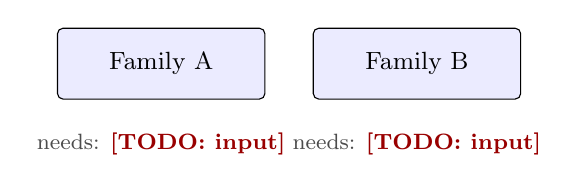
\begin{tikzpicture}[
    fam/.style  = {draw, rounded corners=2pt, align=center, text width=24mm,
                   minimum height=9mm, font=\small, fill=blue!8},
    need/.style = {font=\footnotesize, align=center, text=black!70},
]
  \node[fam]                  (a) {Family A};
  \node[fam, right=6mm of a]  (b) {Family B};
  \node[need, below=3mm of a] {needs: \todo{input}};
  \node[need, below=3mm of b] {needs: \todo{input}};
\end{tikzpicture}
. Keep labels to a few words; explain in the surrounding prose.
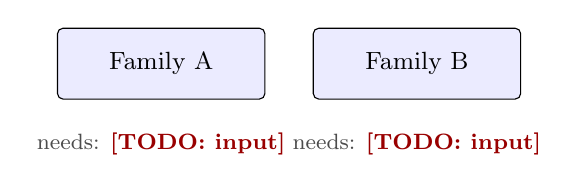
\begin{tikzpicture}[
    fam/.style  = {draw, rounded corners=2pt, align=center, text width=24mm,
                   minimum height=9mm, font=\small, fill=blue!8},
    need/.style = {font=\footnotesize, align=center, text=black!70},
]
  \node[fam]                  (a) {Family A};
  \node[fam, right=6mm of a]  (b) {Family B};
  \node[need, below=3mm of a] {needs: \todo{input}};
  \node[need, below=3mm of b] {needs: \todo{input}};
\end{tikzpicture}

  \caption{Method families and what each needs as input. \todo{Fill in.}}
  \label{fig:taxonomy}
\end{figure}

% Wide table across both columns. Add a row per method (or per group of methods that share
% all four descriptive columns). Never invent an entry: every row needs a reference.
\begin{table*}[t]
\caption{State-of-the-art summary. \todo{Fill in from the literature notes.}}
\label{tab:comparison}
\small
\begin{tabularx}{\textwidth}{@{}L L L L l@{}}
\toprule
\textbf{Measurements used} & \textbf{Estimated quantity} & \textbf{Model used} &
\textbf{Methodology} & \textbf{Ref.}\\
\midrule
\todo{signals} & \todo{quantity} & \todo{model} & \todo{technique} & \cite{singh2019}\\
\addlinespace
\todo{signals} & \todo{quantity} & \todo{model} & \todo{technique} & \todo{ref}\\
\bottomrule
\end{tabularx}
\end{table*}

\subsection{Family A}
\todo{One subsection per family in the taxonomy: the idea in plain words, what it needs, where it
works and where it fails, and which table rows belong to it.}

\subsection{Family B}
\todo{As above.}

\section{Discussion}
\label{sec:discussion}

\todo{What the comparison shows: patterns across the table, which combinations of measurements and
models are well covered, which are thin, and what the sources disagree about.}

\openissue{\todo{Questions the literature does not settle.}}

\paragraph{Limitations of this review.}
\todo{Search coverage, sources not accessible, and the fact that entries come from the papers'
own claims and were not reproduced.}

\section{Conclusion}
\label{sec:conclusion}

\todo{Three to five sentences: what was compared, the main pattern, and what a reader should read
first.}


% References, as a plain thebibliography list so the paper builds with pdflatex alone (no bibtex).
% Numbered in order of first citation. Every entry should be in the literature catalogue,
% ../../study/catalog.md, with its note in ../../study/notes/. Add a new source as another \bibitem.

\begin{thebibliography}{10}

\bibitem{singh2019}
K.~B. Singh, M.~A. Arat, and S.~Taheri.
\newblock Literature review and fundamental approaches for vehicle and tire
  state estimation.
\newblock \emph{Vehicle System Dynamics}, 2019.

\end{thebibliography}


\end{document}
